% Soubory musí být v kódování, které je nastaveno v příkazu \usepackage[...]{inputenc}

\documentclass[%        Základní nastavení
  %draft,    				  % Testovací překlad
  14pt,       				% Velikost základního písma je 12 bodů
	t,                  % obsah slajdů bude vždy začínat od shora (nebude vertikálně centrovaný)
	aspectratio=1610,   % poměr stran bude 16:10 (všechny projektory v učebnách na Technické 12 Brno),
	                    % další volby jsou 43, 149, 169, 54, 32.
	unicode,						% Záložky a informace budou v kódování unicode
]{beamer}				    	% Dokument třídy 'zpráva', vhodná pro sazbu závěrečných prací s kapitolami
%\usepackage{etex}

\usepackage[utf8]		  % Kódování zdrojových souborů je v UTF-8
	{inputenc}					% Balíček pro nastavení kódování zdrojových souborů

\usepackage{graphicx} % Balíček 'graphicx' pro vkládání obrázků
											% Nutné pro vložení logotypů školy a fakulty

\usepackage[          % Balíček 'acronym' pro sazby zkratek a symbolů
	nohyperlinks				% Nebudou tvořeny hypertextové odkazy do seznamu zkratek
]{acronym}
											% Nutné pro použití prostředí 'acronym' balíčku 'thesis'

%% Balíček hyperref je volán třídou beamer automaticky, proto není třeba následujícího kódu:
%\usepackage[
%	breaklinks=true,		% Hypertextové odkazy mohou obsahovat zalomení řádku
%	hypertexnames=false % Názvy hypertextových odkazů budou tvořeny
%											% nezávisle na názvech TeXu
%]{hyperref}						% Balíček 'hyperref' pro sazbu hypertextových odkazů
%											% Nutné pro použití příkazu 'nastavenipdf' balíčku 'thesis'

\usepackage{cmap} 		% Balíček cmap zajišťuje, že PDF vytvořené `pdflatexem' je
											% plně "prohledávatelné" a "kopírovatelné"

%\usepackage{upgreek}	% Balíček pro sazbu stojatých řeckých písmem
											%% např. stojaté pí: \uppi
											%% např. stojaté mí: \upmu (použitelné třeba v mikrometrech)
											%% pozor, grafická nekompatibilita s fonty typu Computer Modern!

%\usepackage{amsmath} %balíček pro sabu náročnější matematiky

\usepackage{booktabs} % Balíček, který umožňuje v tabulce používat
                      % příkazy \toprule, \midrule, \bottomrule


%%%%%%%%%%%%%%%%%%%%%%%%%%%%%%%%%%%%%%%%%%%%%%%%%%%%%%%%%%%%%%%%%
%%%%%%      Definice informací o dokumentu             %%%%%%%%%%
%%%%%%%%%%%%%%%%%%%%%%%%%%%%%%%%%%%%%%%%%%%%%%%%%%%%%%%%%%%%%%%%%

% V tomto souboru se nastavují téměř veškeré informace, proměnné mezi studenty:
% jméno, název práce, pohlaví atd.
% Tento soubor je SDÍLENÝ mezi textem práce a prezentací k obhajobě -- netřeba něco nastavovat na dvou místech.

\usepackage[
  %%% Z následujících voleb jazyka lze použít pouze jednu
  %czech-english,		% originální jazyk je čeština, překlad je anglicky (výchozí)
  %english-czech,	% originální jazyk je angličtina, překlad je česky
  %slovak-english,	% originální jazyk je slovenština, překlad je anglicky
  english-slovak,	% originální jazyk je angličtina, překlad je slovensky
  %
  %%% Z následujících voleb typu práce lze použít pouze jednu
  semestral,		  % semestrální práce (nesází se abstrakty, prohlášení, poděkování) (výchozí)
  %bachelor,			%	bakalářská práce
  %master,			  % diplomová práce
  %treatise,			% pojednání o disertační práci
  %doctoral,			% disertační práce
  %
  %%% Z následujících voleb zarovnání objetů lze použít pouze jednu
  %  left,				  % rovnice a popisky plovoucích objektů budou zarovnány vlevo
  center,			    % rovnice a popisky plovoucích objektů budou zarovnány na střed (vychozi)
  %
]{thesis}   % Balíček pro sazbu studentských prací


%%% Jméno a příjmení autora ve tvaru
%  [tituly před jménem]{Křestní}{Příjmení}[tituly za jménem]
% Pokud osoba nemá titul před/za jménem, smažte celý řetězec '[...]'
\author[Bc.]{Samuel}{Kopecký}

%%% Identifikační číslo autora (VUT ID)
\butid{211799}

%%% Pohlaví autora/autorky
% (nepoužije se ve variantě english-czech ani english-slovak)
% Číselná hodnota: 1...žena, 0...muž
\gender{0}

%%% Jméno a příjmení vedoucího/školitele včetně titulů
%  [tituly před jménem]{Křestní}{Příjmení}[tituly za jménem]
% Pokud osoba nemá titul před/za jménem, smažte celý řetězec '[...]'
\advisor[Ing.]{David}{Smékal}

%%% Jméno a příjmení oponenta včetně titulů
%  [tituly před jménem]{Křestní}{Příjmení}[tituly za jménem]
% Pokud osoba nemá titul před/za jménem, smažte celý řetězec '[...]'
% Nastavení oponenta se uplatní pouze v prezentaci k obhajobě;
% v případě, že nechcete, aby se na titulním snímku prezentace zobrazoval oponent, pouze příkaz zakomentujte;
% u obhajoby semestrální práce se oponent nezobrazuje (jelikož neexistuje)
% U dizertační práce jsou typicky dva až tři oponenti. Pokud je chcete mít na titulním slajdu, prosím ručně odkomentujte a upravte jejich jména v definici "VUT title page" v souboru thesis.sty.
\opponent[TODO]{TODO}{TODO}[TODO]

%%% Název práce
%  Parametr ve složených závorkách {} je název v originálním jazyce,
%  parametr v hranatých závorkách [] je překlad (podle toho jaký je originální jazyk).
%  V případě, že název Vaší práce je dlouhý a nevleze se celý do zápatí prezentace, použijte příkaz
%  \def\insertshorttitle{Zkác.\ náz.\ práce}
%  kde jako parametr vyplníte zkrácený název. Pokud nechcete zkracovat název, budete muset předefinovat,
%  jak se vytváří patička slidu. Viz odkaz: https://bit.ly/3EJTp5A
\title[Modular communication based on post-quantum cryptohraphy]{Modulární komunikace postavená na postkvantové kryptografii}

%%% Označení oboru studia
%  Parametr ve složených závorkách {} je název oboru v originálním jazyce,
%  parametr v hranatých závorkách [] je překlad
\specialization[Information security]{Informačná Bezpečnosť}

%%% Označení ústavu
%  Parametr ve složených závorkách {} je název ústavu v originálním jazyce,
%  parametr v hranatých závorkách [] je překlad
%\department[Department of Control and Instrumentation]{Ústav automatizace a měřicí techniky}
%\department[Department of Biomedical Engineering]{Ústav biomedicínského inženýrství}
%\department[Department of Electrical Power Engineering]{Ústav elektroenergetiky}
%\department[Department of Electrical and Electronic Technology]{Ústav elektrotechnologie}
%\department[Department of Physics]{Ústav fyziky}
%\department[Department of Foreign Languages]{Ústav jazyků}
%\department[Department of Mathematics]{Ústav matematiky}
%\department[Department of Microelectronics]{Ústav mikroelektroniky}
%\department[Department of Radio Electronics]{Ústav radioelektroniky}
%\department[Department of Theoretical and Experimental Electrical Engineering]{Ústav teoretické a experimentální elektrotechniky}
\department[Department of Telecommunications]{Ústav telekomunikací}
%\department[Department of Power Electrical and Electronic Engineering]{Ústav výkonové elektrotechniky a elektroniky}

%%% Označení fakulty
%  Parametr ve složených závorkách {} je název fakulty v originálním jazyce,
%  parametr v hranatých závorkách [] je překlad
%\faculty[Faculty of Architecture]{Fakulta architektury}
\faculty[Faculty of Electrical Engineering and~Communication]{Fakulta elektrotechniky a~komunikačních technologií}
%\faculty[Faculty of Chemistry]{Fakulta chemická}
%\faculty[Faculty of Information Technology]{Fakulta informačních technologií}
%\faculty[Faculty of Business and Management]{Fakulta podnikatelská}
%\faculty[Faculty of Civil Engineering]{Fakulta stavební}
%\faculty[Faculty of Mechanical Engineering]{Fakulta strojního inženýrství}
%\faculty[Faculty of Fine Arts]{Fakulta výtvarných umění}
%
%Nastavení logotypu (v hranatych zavorkach zkracene logo, ve slozenych plne):
\facultylogo[logo/FEKT_zkratka_barevne_PANTONE_CZ]{logo/UTKO_color_PANTONE_CZ}

%%% Rok odevzdání práce
\graduateyear{2023}
%%% Akademický rok odevzdání práce
\academicyear{2022/23}

%%% Datum obhajoby (uplatní se pouze v prezentaci k obhajobě)
\date{14.\,11.\,2022}

%%% Místo obhajoby
% Na titulních stránkách bude automaticky vysázeno VELKÝMI písmeny (pokud tyto stránky sází šablona)
\city{Brno}

%%% Abstrakt
\abstract[%
  Překlad abstraktu
  (v~angličtině, pokud je originálním jazykem čeština či slovenština; v~češtině či slovenštině, pokud je originálním jazykem angličtina)
]{%
  Abstrakt práce v~originálním jazyce
}

%%% Klíčová slova
\keywrds[%
  Překlad klíčových slov
  (v~angličtině, pokud je originálním jazykem čeština či slovenština; v~češtině či slovenštině, pokud je originálním jazykem angličtina)
]{%
  Klíčová slova v~originálním jazyce
}

%%% Poděkování
\acknowledgement{%
  Rád bych poděkoval vedoucímu bakalářské/diplomové/disertační práce
  panu Ing.~XXX YYY, Ph.D.\ za odborné vedení,
  konzultace, trpělivost a~podnětné návrhy k~práci.
}%      % v tomto souboru doplňte údaje o sobě, o názvu práce...
                       % (tento soubor je sdílený s textem práce)


%%%%%%%%%%%%%%%%%%%%%%%%%%%%%%%%%%%%%%%%%%%%%%%%%%%%%%%%%%%%%%%%%%%%%%%%

%%%%%%%%%%%%%%%%%%%%%%%%%%%%%%%%%%%%%%%%%%%%%%%%%%%%%%%%%%%%%%%%%%%%%%%%
%%%%%%     Nastavení polí ve Vlastnostech dokumentu PDF      %%%%%%%%%%%
%%%%%%%%%%%%%%%%%%%%%%%%%%%%%%%%%%%%%%%%%%%%%%%%%%%%%%%%%%%%%%%%%%%%%%%%
%% Při vloženém balíčku 'hyperref' lze použít příkaz '\pdfsettings'
\pdfsettings
%  Nastavení polí je možné provést také ručně příkazem:
%\hypersetup{
%  pdftitle={Název studentské práce},    	% Pole 'Document Title'
%  pdfauthor={Autor studenstké práce},   	% Pole 'Author'
%  pdfsubject={Typ práce}, 						  	% Pole 'Subject'
%  pdfkeywords={Klíčová slova}           	% Pole 'Keywords'
%}
\hypersetup{pdfpagemode=FullScreen}       % otevření rovnou v režimu celé obrazovky
%%%%%%%%%%%%%%%%%%%%%%%%%%%%%%%%%%%%%%%%%%%%%%%%%%%%%%%%%%%%%%%%%%%%%%%

\usetheme{VUT} 				% barvy a rozložení prezentace odpovídající VUT FEKT
% alternativně lze použít jiná berevná témata, ale bez záruky. Například:
%\usetheme{Darmstadt} \usecolortheme{default2}
\logoheader					% vytvoření zkráceného loga VUT FEKT v hlavičce slajdu, nechte odkomentované


\begin{document}

% v případě zakomentování následujícího se zobrazí v pravém dolním rohu slajdů klikatelné navigační symboly
\disablenavigationsymbols


% titulní snímek, vysazen bez horních, dolních a postranních lišt (volba plain),
% není tak vysazen ani nadpis snímku
\maketitle
\newcommand{\npm}[2]{{#1}\,$\pm\,{#2}\%$}

\begin{frame}[c]
	\frametitle{Ciele práce}
	\large{\begin{itemize}
			\item Optimalizácia post kvantových algoritmov
			\item Protokol na výmenu dát z zabepečeným post kvantovou kryptografiou
			\item Systém modularity kryptografických algoritmov
			\item Textové terminálové rozhranie
			\item Grafické terminálové rozhranie -- TUI
		\end{itemize}
	}
\end{frame}

\begin{frame}[c]
	\frametitle{Post kvantové algoritmy}
	\begin{columns}[T]
		\begin{column}{0.8\textwidth}
			\large{\begin{itemize}
					\item Algoritmus výmenu tajného klúča -- Kyber
					\item Algoritmus digitálneho podpisu -- Dilithium
					\item NIST štandardrizované algoritmy
					\item Implementácia v jazyku Go (Golang)
					\item Výsledky implementácie porovnávané z kničnicou Circl od Cloudflare
				\end{itemize}
			}
		\end{column}
		\begin{column}{0.2\textwidth}
			\begin{figure}
				
\includegraphics[width=\linewidth]{presentation_pictures/Golang_Logo.png}
			\end{figure}
		\end{column}
	\end{columns}
\end{frame}

\begin{frame}[c]
	\frametitle{Výsledky implementácie}
	\large{
		\begin{itemize}
			\item Testované na AMD 3600 s frekvenciou jadra 3.6\,Ghz
		\end{itemize}
	}
	\normalsize{
		\begin{table}[h!]
			\centering
			\begin{tabular}{|l|r|r|}
  \hline
             & PqCom [\textmu s] & Circl [\textmu s] \\
  \hline
  \hline
  Kyber512   & \npm{459.9}{1}    & \npm{109.7}{2}    \\
  Kyber768   & \npm{707.9}{1}    & \npm{171.7}{2}    \\
  Kyber1024  & \npm{1019}{1}     & \npm{267.4}{2}    \\
  \hline
  Dilithium2 & \npm{1986}{1}     & \npm{472.9}{1}    \\
  Dilithium3 & \npm{3206}{2}     & \npm{788.1}{0}    \\
  Dilithium5 & \npm{4130}{1}     & \npm{1054}{1}     \\
  \hline
\end{tabular}

		\end{table}
	}
\end{frame}

\begin{frame}[c]
	\frametitle{Protokol sieťovej komunikácie}
	\large{\begin{itemize}
			\item Založený na protokole TCP, predvolený port 4040
			\item Zabezpečený len post kvantovou kryptografiou
			\item Šifrovanie a integrita zaistená pomcou AES-256-GCM
			\item Algoritmy pre výmna klúča a digitálny podpis sú modulárne
			\item Používa fixnú velkosť hlavičky ktorá ma iba 3\,B
		\end{itemize}}
	\begin{figure}
		
\includegraphics[width=.8\textwidth]{presentation_pictures/header_sk.pdf}
	\end{figure}
\end{frame}

\begin{frame}[c]
	\frametitle{Protokol sieťovej komunikácie}
	\large{\begin{itemize}
			\item Typ určuje štruktúru správy, existujú 4 typy správ
			      \begin{itemize}
				      \large{\item \texttt{ClientInitT}}
				            \large{\item \texttt{ServerInitT}}
				            \large{\item \texttt{ContentT}}
				            \large{\item \texttt{ErrorT}}
			      \end{itemize}
			\item Existuje podpora pre dalších 251 typov
		\end{itemize}}
\end{frame}

\begin{frame}[c]
	\frametitle{Protokol sieťovej komunikácie}
	\begin{figure}
		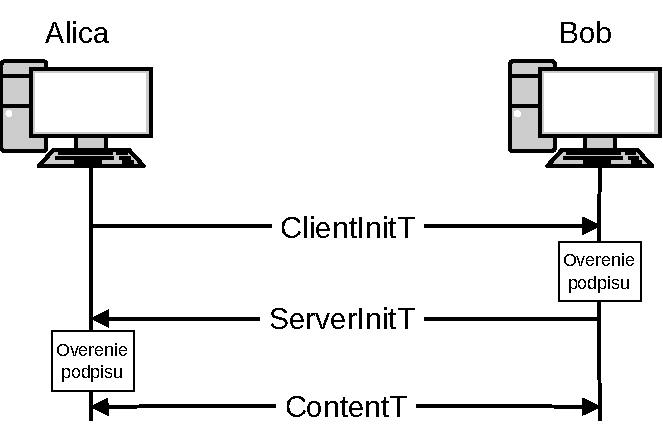
\includegraphics[width=.8\textwidth]{presentation_pictures/comm.pdf}
	\end{figure}
\end{frame}

\begin{frame}[c]
	\frametitle{Protokol sieťovej komunikácie}
	\large{\begin{itemize}
			\item Klient pošle svôj verejný klúč a podpíše správu
			\item Server overí podpis, zašifruje súkromný klúč a podpíše správu
			\item Klient overý podpis, dešifruje súkromný klúč
			\item Začne šifrovaná komunikácia pomocou súkromného klúča
		\end{itemize}
	}
\end{frame}

\begin{frame}[c]
	\frametitle{Modularita algoritmov}
	\large{\begin{itemize}
			\item Algoritmy sa volia pomocou konfiguračných súborov
			\item Konfiguračné súbory naďalej obsahujú verejný a súkromný klúč
			\item Algoritmy sa musia rovnať pri vzájomnej komunikácií
			\item Možno dodať ďalšie algoritmy z minimálnou zmenou v kóde
		\end{itemize}}
\end{frame}

\begin{frame}[c]
	% bez nadpisu snímku
	\frametitle{\mbox{ }}
	\begin{center}
		{\Huge Ukážka aplikácie v TUI}
	\end{center}
\end{frame}

\begin{frame}[c]
	\frametitle{Chyba v konfigurácií}
	\begin{figure}
		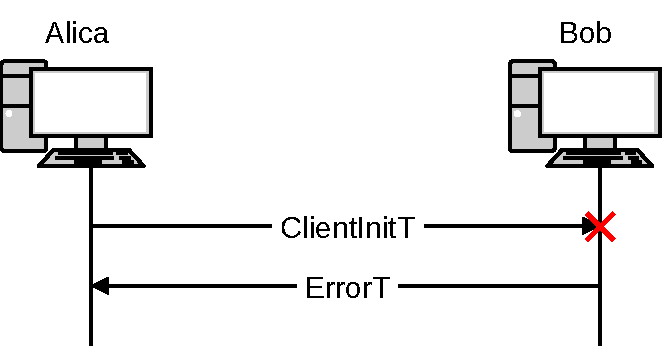
\includegraphics[width=.9\textwidth]{presentation_pictures/comm_err.pdf}
	\end{figure}
\end{frame}

\begin{frame}[c]
	\frametitle{Chyba v konfigurácií}
	\begin{figure}[htbp]
		\centering
		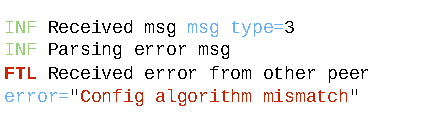
\includegraphics[width=\textwidth]{presentation_pictures/client_err.pdf}
	\end{figure}
\end{frame}

\begin{frame}[c]
	\frametitle{Ďalšie vlastnosti aplikácie}
	\large{\begin{itemize}
			\item Program informuje uživatela o dalších informáciach pomocou log správ
			\item Ukladanie log správ do súboru počas TUI
			\item Integrácia z UNIX textovým rozhraním (presmerovanie \texttt{stdout}, \texttt{stdin})
			\item Ochrana proti útokom s opakovaním správ pomocou cookie
			\item Integrácia analýzi vo wiresharku pomocou \texttt{lua} skriptu
			\item Podpora Windows aj Unix systémoch
		\end{itemize}}
\end{frame}

% podekovani
\begin{frame}[c]
	% bez nadpisu snímku
	\frametitle{\mbox{ }}
	\begin{center}
		{\Huge Ďakujem za pozornosť!}
	\end{center}
\end{frame}

% otázky oponenta
% \frame{
% \frametitle{Otázky oponenta}
% 	\emph{Jaká je souvislost Vašeho vzorce (1.2) s~Maxwellovými rovnicemi v~integrálním tvaru?}\\[2ex]
% 	%
% 	Již staří Římané\,\dots
% }

\end{document}
